% !TEX TS-program = pdflatexmk

\documentclass[modern,linenumbers]{aastex61}

\usepackage{acronym}
\usepackage{amsmath}
\usepackage{amssymb}

\newcommand{\chieff}{\chi_\mathrm{eff}}
\newcommand{\dd}{\mathrm{d}}
\newcommand{\diff}[2]{\frac{\dd #1}{\dd #2}}
\newcommand{\fixme}[1]{\textcolor{red}{FIXME: #1}}
\newcommand{\pali}{p_\mathrm{ali}}
\newcommand{\piso}{p_\mathrm{iso}}

\newcommand{\checkme}[1]{\textcolor{red}{#1}}

\newcommand{\OOneSigmaIsoAligned}{\checkme{1.7}}
\newcommand{\OOneOddsIsoAligned}{\checkme{0.087}}
\newcommand{\OTwoSigmaIsoAlignedMin}{\checkme{3.0}}
\newcommand{\OTwoOddsIsoAlignedMin}{\checkme{0.0012}}

\newcommand{\ilya}[1]{\textcolor{purple}{#1}}
\newcommand{\will}[1]{\textcolor{cyan}{#1}}

\begin{document}

\acrodef{BBH}{binary black hole}
\acrodef{BH}{black hole}
\acrodef{EM}{electromagnetic}
\acrodef{GW}{gravitational wave}
\acrodef{PE}{parameter estimation}

\title{Distinguishing Between Spin-Aligned and Isotropic Binary Black
  Hole Populations Using Gravitational Wave Observations}

\author[0000-0003-1540-8562]{Will M. Farr}

\affiliation{Birmingham Institute for Gravitational Wave Astronomy and
  School of Physics and Astronomy, University of Birmingham,
  Birmingham, B15 2TT, United Kingdom}

\author[0000-0002-6100-537X]{Simon Stevenson}

\affiliation{Birmingham Institute for Gravitational Wave Astronomy and
  School of Physics and Astronomy, University of Birmingham,
  Birmingham, B15 2TT, United Kingdom}

\author{M. Coleman Miller}

\affiliation{Department of Astronomy and Maryland Center for Theory
  and Computation, University of Maryland, College Park MD
  20742, United States}

\author[0000-0002-6134-8946]{Ilya Mandel}

\affiliation{Birmingham Institute for Gravitational Wave Astronomy and
  School of Physics and Astronomy, University of Birmingham,
  Birmingham, B15 2TT, United Kingdom}

\author[0000-0002-6254-1617]{Alberto Vecchio}

\affiliation{Birmingham Institute for Gravitational Wave Astronomy and
  School of Physics and Astronomy, University of Birmingham,
  Birmingham, B15 2TT, United Kingdom}

\email{w.farr@bham.ac.uk,simons@star.sr.bham.ac.uk,miller@astro.umd.edu,imandel@star.sr.bham.ac.uk,av@star.sr.bham.ac.uk}

\begin{abstract}
  The first direct detections of \acp{GW} from merging \acp{BBH} open
  a unique window into the formation environment of massive stars and
  their compact remnants.  One promising signature of the formation
  environment is the angular distribution of the \ac{BH} spins;
  systems formed through dynamical interacions among already-compact
  objects are expected to have isotropic spin orientations while
  binaries formed from pairs of stars born together are more likely to
  have spins aligned with the binary orbit as a consequence of their
  joint evolution toward a \ac{BBH} system.  By considering existing
  \ac{GW} measurements of $\chieff$, the best-measured combination of
  spin parameters, in the three likely binary black hole detections
  GW150914, LVT151012, and GW151226, we show that the data already
  exhibit a $\OOneSigmaIsoAligned\sigma$ ($\OOneOddsIsoAligned$ odds
  ratio) preference for an isotropic angular distribution amongst a
  suite of models for the spin distribution.  By considering the
  effect of an additional 10 detections drawn from the various models
  in the suite we show that such an agumented data set would enable at
  least a $\OTwoSigmaIsoAlignedMin\sigma$ ($\OTwoOddsIsoAlignedMin$
  odds ratio) distinction between the isotropic and aligned models,
  and in most cases better than $5\sigma$ ($2.9 \times 10^{-7}$ odds
  ratio).  The existing data strongly suggest a dynamical formation
  secnario for the observed systems, and this will be confirmed (or
  overturned) confidently in the near future by subsequent
  observations.
\end{abstract}

\acresetall{}

\section{\ac{GW} Spin Measurements and Model Selection}
\label{sec:O1}

Following the detection of a merging \ac{BBH} system, \ac{PE} tools
\citep{2015PhRvD..91d2003V} compare model gravitational waveforms
\citep{2014PhRvD..89h4006P,2014PhRvD..89f1502T,2014PhRvL.113o1101H}
against the observed data to obtain a posterior distribution on the
parameter space that describes the compact binary source.  The spin
parameter with the largest effect on waveforms, and a correspondingly
tight constraint from the data, is a mass-weighted, aligned,
``effective spin,''
\begin{equation}
  \chieff = \frac{c}{GM} \left( \frac{\vec{S}_1}{m_1} + \frac{\vec{S}_2}{m_2}
  \right) \cdot \frac{\vec{L}}{\hat{L}} = \frac{1}{M} \left( m_1 a_1^z + m_2 a_2^z \right),
\end{equation}
where the $\hat{z}$ axis is aligned with the orbital angular momentum
of the binary, $m_{1,2}$ are the masses of the more-massive (1) and
less-massive (2) components, $M = m_1 + m_2$ is the total mass,
$\vec{S}_{1,2}$ are the spin angular momentum vectors of the black
holes in the binary, $\vec{L}$ is the orbital angular momentum vector,
and $a_{1,2}$ are the corresponding dimensionless spin parameters
\citep{2016PhRvL.116x1102A}.

Figure \ref{fig:O1-posteriors} shows an approximation to the posterior
inferred on $\chieff$ for the three likely \ac{GW} detections
GW150914, GW151226 and LVT151012 from \citet{O1-BBH}.  Because samples
drawn from the posterior on $\chieff$ are not publicly released at
this time, we have approximated the posterior as a Gaussian
distribution with the same mean and 90\% credible interval as quoted
in \citet{O1-BBH}.  There is essentially no posterior support for
$\chieff \gtrsim 0.5$ as observed in the majority of the
electromagnetically-detected stellar-mass black hole population.

\begin{figure}
  \plotone{../plots/chi-eff-mock-posteriors}
  \caption{\label{fig:O1-posteriors} Approximate posteriors on
    $\chieff$ from the LIGO O1 observations in \citet{O1-BBH}.  We
    approximate the posteriors reported in \citet{O1-BBH} using
    Gaussians with the same median and 90\% credible interval as
    reported in \citet{O1-BBH}.  It is notable that none of the
    $\chieff$ posteriors extends to the high spins in
    electromagnetically-detected stellar-mass black hole systems
    \citep{2015PhR...548....1M}.}
\end{figure}

Small values of $\chieff$ can result from either intrinsically small
spins or larger spins whose direction is mis-aligned with the orbital
plane of the binary (i.e.\ spin vectors with with small
$z$-components).  Mis-alignment is capable of producing
\emph{negative} values of $\chieff$, however, while small, aligned
spins will always have $\chieff \geq 0$.  To quantify the degree of
support for these two alternate explanations of small $\chieff$ values
in the merging \ac{BBH} population, we compared the Bayesian evidence
for various simple models of the spin population using the \ac{GW}
data set.  

Each of our models for the merging \ac{BBH} spin population assumes
that the merging black holes are of equal mass (this is marginally
consistent with the three observations \citep{O1-BBH}, and the
$\chieff$ distribution is not particularly sensitive to the mass ratio
between the merging objects---see Section \ref{sec:mass-ratio}).  We
assume that the population spin distribution factorises into a
distribution for the spin magnitude, $a$, and a distribution for the
spin angles.  Finally, we assume that the distribution of spins is
common to each component in a merging binary.  Choosing one of three
magnitude distributions
\begin{equation}
  \label{eq:magnitude-dists}
  p(a) = \begin{cases}
    2\left(1-a\right) & \textnormal{``decreasing''} \\
    1 & \textnormal{``flat''} \\
    2\left(a-1\right) & \textnormal{``increasing''}
  \end{cases},
\end{equation}
and pairing with either an isotropic angular distribution or a
distribution that generates perfect alignment with the positive $z$
axis yields six different models for the $\chieff$ distribution.
These models are shown in Figure \ref{fig:chieff-distribution-models}.

\begin{figure}
  \plotone{../plots/chi-eff-distributions}
  \caption{\label{fig:chieff-distribution-models} The models for the
    distribution of $\chieff$ considered in this paper.  In all models
    we assume that the binary mass ratio $q \equiv m_1/m_2 = 1$ and
    that the same distribution of spin vectors obtains for each
    component.  The ``flat'' (blue lines), ``increasing,'' (green
    lines), and ``decreasing'' (red lines) magnitude distributions are
    defined in Eq.\ \eqref{eq:magnitude-dists}.  Solid lines give the
    $\chieff$ distribution under the assumption that the orientations
    of the spins are isotropic; dashed lines give the distribution
    under the assumption that both objects' spins are aligned with the
    orbital angular momentum.  The isotropic distributions are readily
    distinguished from the aligned by the production of negative
    $\chieff$ values, while the distinction between the three models
    for the spin magnitude distribution is less sharp.}
\end{figure}

We fit hierarchical models of the three LIGO O1 observations using
these six different, zero-parameter population distributions (see
Section \ref{sec:hierarchical}).  We also fit three mixture models for
the population, where the spin magnitude distribution is fixed but the
angular distribution is a weighted sum of the isotropic and aligned
distribution.  The evidence, or marginal likelihood, for each of the
models is shown in Figure \ref{fig:O1-odds}.  For all three magnitude
distributions, the mixture models' posterior on the mixing fraction
peaked at 100\% isotropic, explaining why the zero-parameter,
pure-isotropic models are preferred over the single-parameter mixture
models for every magnitude distribution with this data set.  Not
surprisingly, given the small $\chieff$ values in the three detected
systems, the most-favoured model among those with an isotropic angular
distribution has the ``decreasing'' magnitude distribution; the most
favoured model among those with an aligned distribution also has the
``decreasing'' magnitude distribution.  The odds ratio between the
aligned and isotropic models is $\OOneOddsIsoAligned$, or
$\OOneSigmaIsoAligned\sigma$; thus the data strongly favour isotropic
spins among our suite of models.

\begin{figure}
  \plotone{../plots/Wills_evidence_ratio_figure_with_mixture_models.png}
  \caption{Odds ratios among our models using the approximations to
    the posteriors on $\chieff$ from the O1 observations shown in
    Figure \ref{fig:O1-posteriors}.  The flat (``F''), increasing
    (``I''), and decreasing (``D'') spin magnitude distributions (see
    Eq.\ \eqref{eq:magnitude-dists}) are paired with isotropic,
    aligned angular distributions (``$\mathrm{I}$'',
    ``$\mathrm{A}$''), as well as a mixture model of the two
    (``$\mathrm{M}$'').  The most-favoured models have a decreasing
    distribution of spin magnitudes.  The odds ratio between these
    models is $\OOneOddsIsoAligned$, or $\OOneSigmaIsoAligned\sigma$.
    For all magnitude distributions the pure-isotropic models are
    preferred over the mixture models; correspondingly, the posterior
    on the mixture fraction peaks at 100\% isotropic.}
  \label{fig:O1-odds}
\end{figure}

\subsection{Future Spin Measurements}
\label{subsec:future}

Estimates of the rate of \ac{BBH} coalescences give a reasonable
chance of 10 additional \ac{BBH} detections in the near future
\citep{O1-BBH,2016ApJ...833L...1A,2016ApJS..227...14A}.  Assuming an
additional 10 detections drawn from each of our six zero-parameter
models for the spin distribution, we find the odds ratios shown in
Figure \ref{fig:O2-predictions}.  We find that most scenarios with an
additional 10 detections allow to distinguish the correct angular
distribution with greater than $5\sigma$ ($2.9 \times 10^{-7}$ odds)
credibility; and in the worst case the distinction is
$\OTwoSigmaIsoAlignedMin\sigma$ ($\OTwoOddsIsoAlignedMin$ odds ratio).

\begin{figure}
  \plotone{../plots/six-way-O2-model-selection}
  \caption{\label{fig:O2-predictions} Distribution of odds ratios
    predicted with 10 additional observations above the three
    discussed in Section \ref{sec:O1}.  Each panel corresponds to
    additional observations drawn from one of the $\chieff$
    distribution models.  The model from which the additional
    observations are drawn is outlined in red.  The height of the blue
    bar gives the median odds ratio relative to the model from which
    the additional observations are drawn; the green line gives the
    68\% ($1 \sigma$) symmetric interval of odds ratios over 1000
    separate draws from the model distribution.  The closest ratio
    between the most-favoured isotropic model and the most-favoured
    aligned model is $\OTwoOddsIsoAlignedMin$, corresponding to
    $\OTwoSigmaIsoAlignedMin\sigma$ preference for the correct angular
    distribution; most models result in more than $5\sigma$ preference
    for the correct angular distribution.  Because the three
    observations from Section \ref{sec:O1} are included in each data
    set the ``correct'' model is not necessarily preferred over the
    others, particularly when that model uses the ``increasing''
    magnitude distribution, which is strongly dis-favoured from the O1
    observations alone.}
\end{figure}

\section{Discussion}

Most of our resolving power for the spin angular distribution is a
result of the fact that our ``aligned'' models cannot produce
$\chieff < 0$ (see Figure \ref{fig:chieff-distribution-models}).  If
spins are intrinsically very small, with $a \lesssim 0.1$ always, then
it is no longer possible to resolve the negative spin with a small
number of observations.  As noted below, however, spins observed in
X-ray binaries are generally large, and most models of isolated binary
evolution do not produce systems with spins uniformly bounded to small
values.

\citet{2017CQGra..34cLT01V} also studied the possibility of
distinguishing aligned and isotropic angular distributions of \ac{BBH}
spins, but concluded that several hundred sources would be required to
adequately separate the models.  The ``aligned'' population in that
study permitted spins nearly parallel or anti-parallel to the orbital
axis, i.e.\ $\hat{S}\cdot \hat{L} \simeq \pm 1$, in contrast to our
aligned models.  Anti-parallel spins are strongly disfavoured in
models of isolated binary evolution.  \ilya{This would be a good place
  for some review articles about pop.\ synth.}

In order to perform our analysis we need to select models for the
distribution of the dimensionless spin parameters of stellar-mass
black holes.  Data for such model selection is sparse.
\citet{2015PhR...548....1M} give current estimates of the spin
parameters for stellar-mass black holes, obtained using disk
reflection and/or disk continuum methods.

Most of the systems studied are low-mass X-ray binaries (i.e., the
donor star has a mass $M_{\rm donor}<1~M_\odot$) rather than the
high-mass X-ray binaries that are likely to be the progenitors of
double black hole binaries.  In addition, there are substantial
systematic errors that can complicate either type of analysis (see
\citealt{2015PhR...548....1M} for a discussion). Nonetheless, if we
take the reported spin magnitudes as representative then we find that
there is a preference for high spins; for example, 14 of the 19
systems with reported spins have spin parameters in excess of 0.5.
The masses and spin parameters of stellar-mass black holes are
unlikely to be altered significantly by accretion (low-mass donors
simply do not have enough mass and high-mass donors have a very short
phase in which they transfer mass; a variant of this long-standing
argument was presented by \citet{1999MNRAS.305..654K}).  Thus the
current spin parameters probably are close to their values upon core
collapse.  We emphasize, however, that the specific processes involved
in the production of black hole binaries could alter the spin
distribution of those holes: for example, close tidal interactions
could spin up the core, or stripping of the envelope could reduce the
available angular momentum.

With this in mind, we performed our analysis using three straw-man
spin distributions for spin parameters from $a/M=0$ to 1: flat
($P(a/M)=1$); rising ($P(a/M)=2a/M$); and falling ($P(a/M)=2(1-a/M)$).
These are not meant to represent any particular physical model, and
indeed neither observations nor population synthesis codes can
authoritatively suggest {\it any} particular spin distribution.  This
does, however, allow us to see how sensitive the $\chieff$
distribution is to spin alignment models given uncertainties about the
spin magnitudes.

Although BH spin-orbit alignment is assumed in continuum flux
measurements \citep{2015PhR...548....1M}, some BH XRBs, including GRO
J1655-40 \ilya{and 4U 1543-475?} appear to indicate that the micro
quasar jet, presumably aligned with the BH spin axis, is misaligned
with the orbit.  Moreover, initial stellar spins in massive binaries
have been observed to be misaligned \ilya{[ref]}, though there are
opportunities for realignment during binary evolution, as described
below.

There are a few modelling constrains on the predicted spin
distribution.  We separate these into a discussion of spin magnitudes
and spin directions (spin-orbit misalignment angles) as in the
preceding analysis; however, it is worth pointing out that, contrary
to our simplified assumptions, the magnitude and direction
distributions may well be coupled.

Several models for binary black hole formation have been proposed
\citep[e.g.,][]{2016ApJ...818L..22A}, yielding potentially different spin
distributions.

The spin directions of binary black holes formed dynamically through
interactions in dense stellar environments \ilya{[add refs. if not
  discussed elsewhere]} are expected to be isotropic given the absence
of a preferred direction \citep[e.g.,][]{2016ApJ...832L...2R} and the
persistence of an isotropic distribution through post-Newtonian
evolution \citep{2004PhRvD..70l4020S}.

Chemically homogeneous evolution is a possible BBH formation channel
specific to rapidly spinning massive stars aligned by tidal effects
\ilya{[add refs. if not discussed elsewhere]}.  However, wind-driven
mass loss can spin down even some of these stars to the point that
values of $\chi_\textrm{eff}$ as low as $\sim 0.2$ are possible,
though alignment should be preserved \citep{2016AnA...588A..50M}.

The classical isolated binary evolution channel through the
common-envelope (CE) phase \ilya{[add refs. if not discussed
  elsewhere]} yields the following typical formation channel for
binary black holes: possible mass transfer from the primary to the
secondary; the collapse of the primary into a BH; the formation and
ejection of a CE as a consequence of dynamically unstable mass
transfer from the secondary to the primary; possible further mass
transfer from remaining secondary core to primary; collapse of the
secondary into a BH; a merger induced by GW emission
\citep[e.g.,][]{2016Natur.534..512B,Stevenson:2017}.  Interaction
before the collapse of the primary could realign the binary, but the
primary’s spin in the wide (separation $\gtrsim 10$ AU) binary can
easily be misaligned by even moderate \citep{2015MNRAS.450L..85M}
natal kicks.  Realignment of the primary through subsequent mass
accretion is unlikely given the small amount of accreted mass, except
perhaps during hyper-critical accretion during CE \ilya{[add ref. to
  Linden?]}; realignment through dissipation in the possibly warped
accretion disk \citep{1975ApJ...195L..65B} is possible, but calculations
suggest it is unlikely for stellar-mass binaries \citep{KLOP}.

The secondary should tidally align with the orbit before the onset of
mass transfer
\citep[e.g.,][]{2000ApJ...541..319K,2013PhRvD..87j4028G}; however,
most of its angular momentum would be lost to the envelope, which will
be ejected during the CE phase.  The remnant core may or may not be
efficiently re-aligned, depending on the separation between the
secondary’s core and the BH immediately after the CE is ejected
\citep{2016MNRAS.462..844K}.  The secondary’s natal kick will be small
relative to the orbital velocity of the close post-CE binary, so any
further kick-induced misalignment will be moderate
\citep{2016ApJ...832L...2R}.

The analysis above assumed the conservation of angular momentum during
core collapse. However, we know that this may not always be the case.
For example, the magnitude of the angular momentum cannot possibly be
conserved during the collapse to a BH if the pre-collapse
dimensionless spin exceeds $1$.  The direction of the angular momentum
may also change; for example, the misalignment of the secondary pulsar
in the double pulsar \ilya{J0737} by $\sim 135^{\circ}$ relative to
the orbit in the apparent absence of a kick indicated that, at least
for slowly spinning objects, a spin tilt during a supernova may be
possible \citep{2011ApJ...742...81F}.  The dependence of the magnitude
and direction of the spin on its pre-collapse values depends on the
stellar structure (i.e., the level of angular momentum coupling
between the collapsing and ejected material), the supernova explosion
(if any), and the details of the post-collapse fallback process
\ilya{[Check if Levin and Matzner are done]}.

In short, the angular distribution of spins in \acp{BBH} formed
through isolated binary evolution is uncertain; nevertheless, it is
more probable that spins are aligned and non-zero after evolution
through this channel than not.  


\appendix

\section{Mixture model}

BBHs can form as the end point of isolated binary evolution \cite{refs}, or dynamically in dense stellar environments \cite{refs}. The spin misalignments of BBHs is a signature of their formation mechanism; binaries formed through isolated binary evolution are expected to have their spins aligned with the orbital angular momentum, whilst those formed dynamically are expected to have an isotropic distribution.

Rate uncertainties for both of these formation scenarios are large enough that we do not know a priori which will dominate the LIGO detection rate. In the previous section we have shown that a model with isotropic spin directions and 'decreasing' spin magnitudes is favoured by the data.

In this section we assume that the true distribution of BBH spin-orbit misalignments observed by LIGO is a mixture of binaries formed through isolated binary evolution (with aligned spins) and dynamical formation (with isotropic spins). 

%
\begin{figure}
\centering
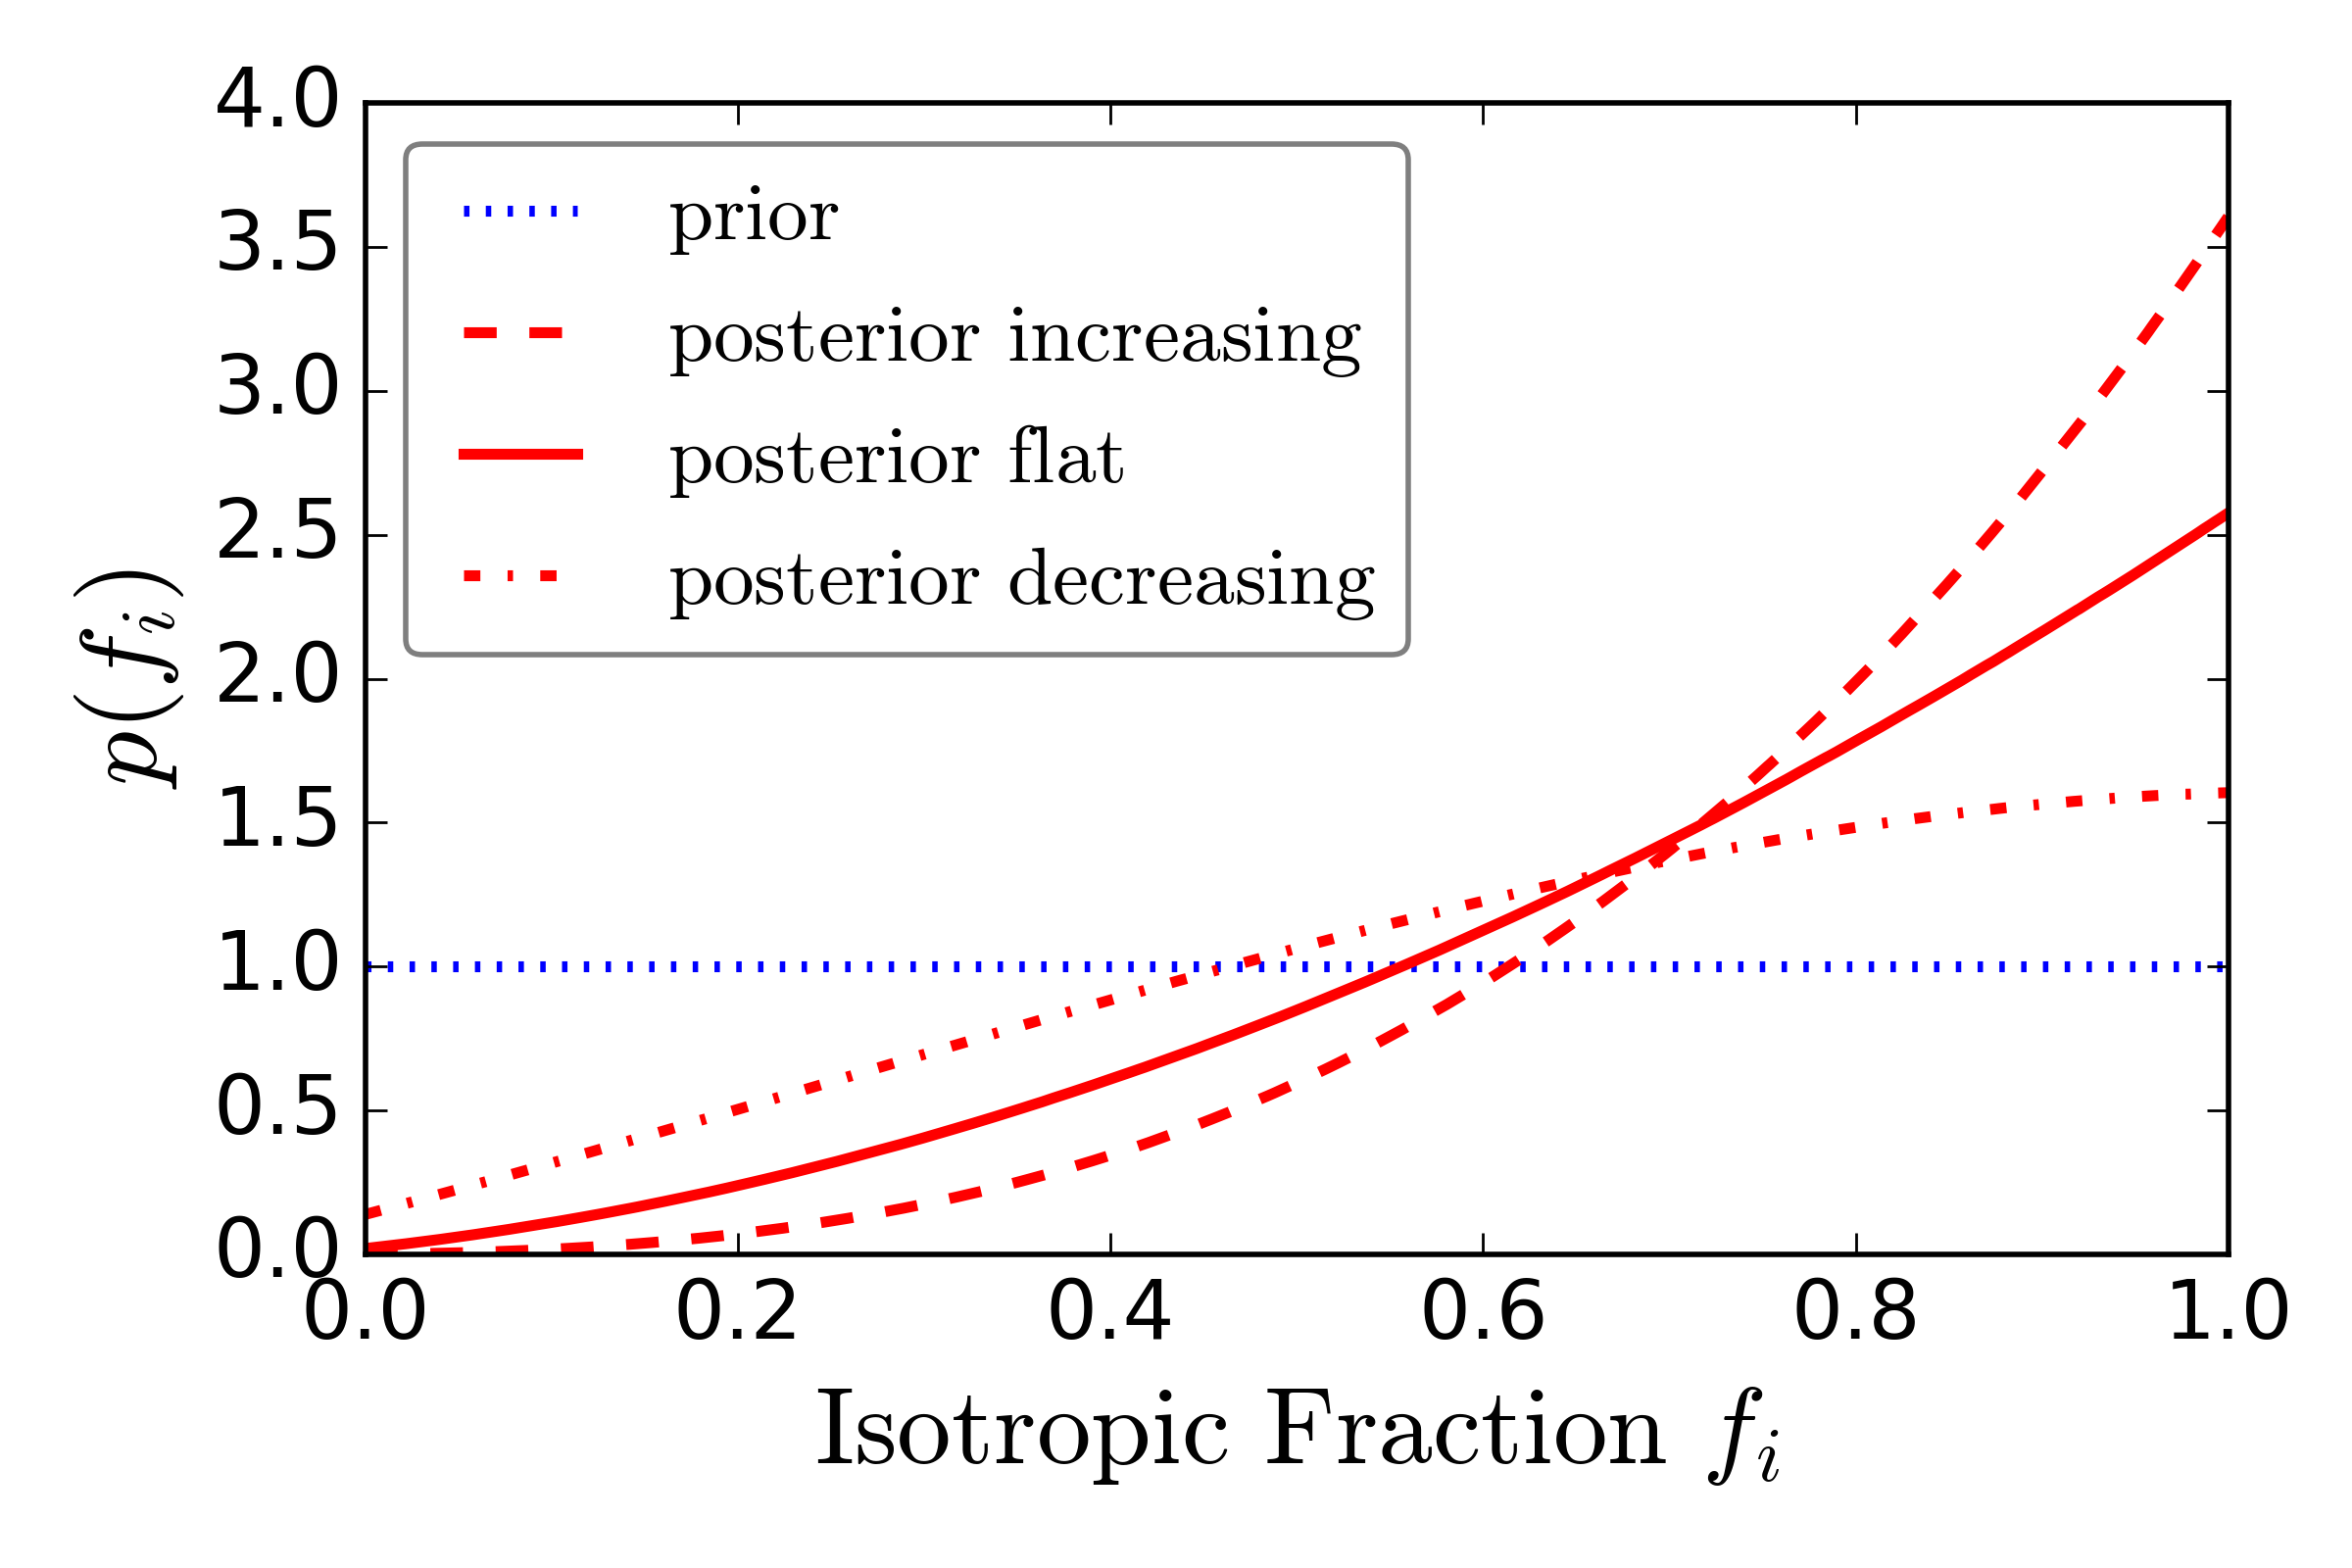
\includegraphics[width=0.45\textwidth]{../plots/posterior_on_isotropic_fraction.png}
\caption{\textbf{Fraction of the BBH population coming from an isotropic distribution} The dotted (blue) line shows the flat prior on the fraction of BBHs coming from an isotropic distribution $f_i$. The solid (red) line shows the posterior after O1, assuming that all BHs have their spin magnitude drawn from a uniform distribution. The dashed line assumes a `increasing' distribution $p(a) = 2a$ for BH spin magnitudes, whilst the dot-dash line assumes a `decreasing' distribution $p(a) = 2(1-a)$. We see that regardless of our assumption regarding BH spin magnitudes, there is a preference for a large fraction coming from an isotropic distribution.}
\label{fig:mixture_fraction_posterior}
\end{figure}
%

%-- could also use the cumulative posterior
%%
%\begin{figure}
%\centering
%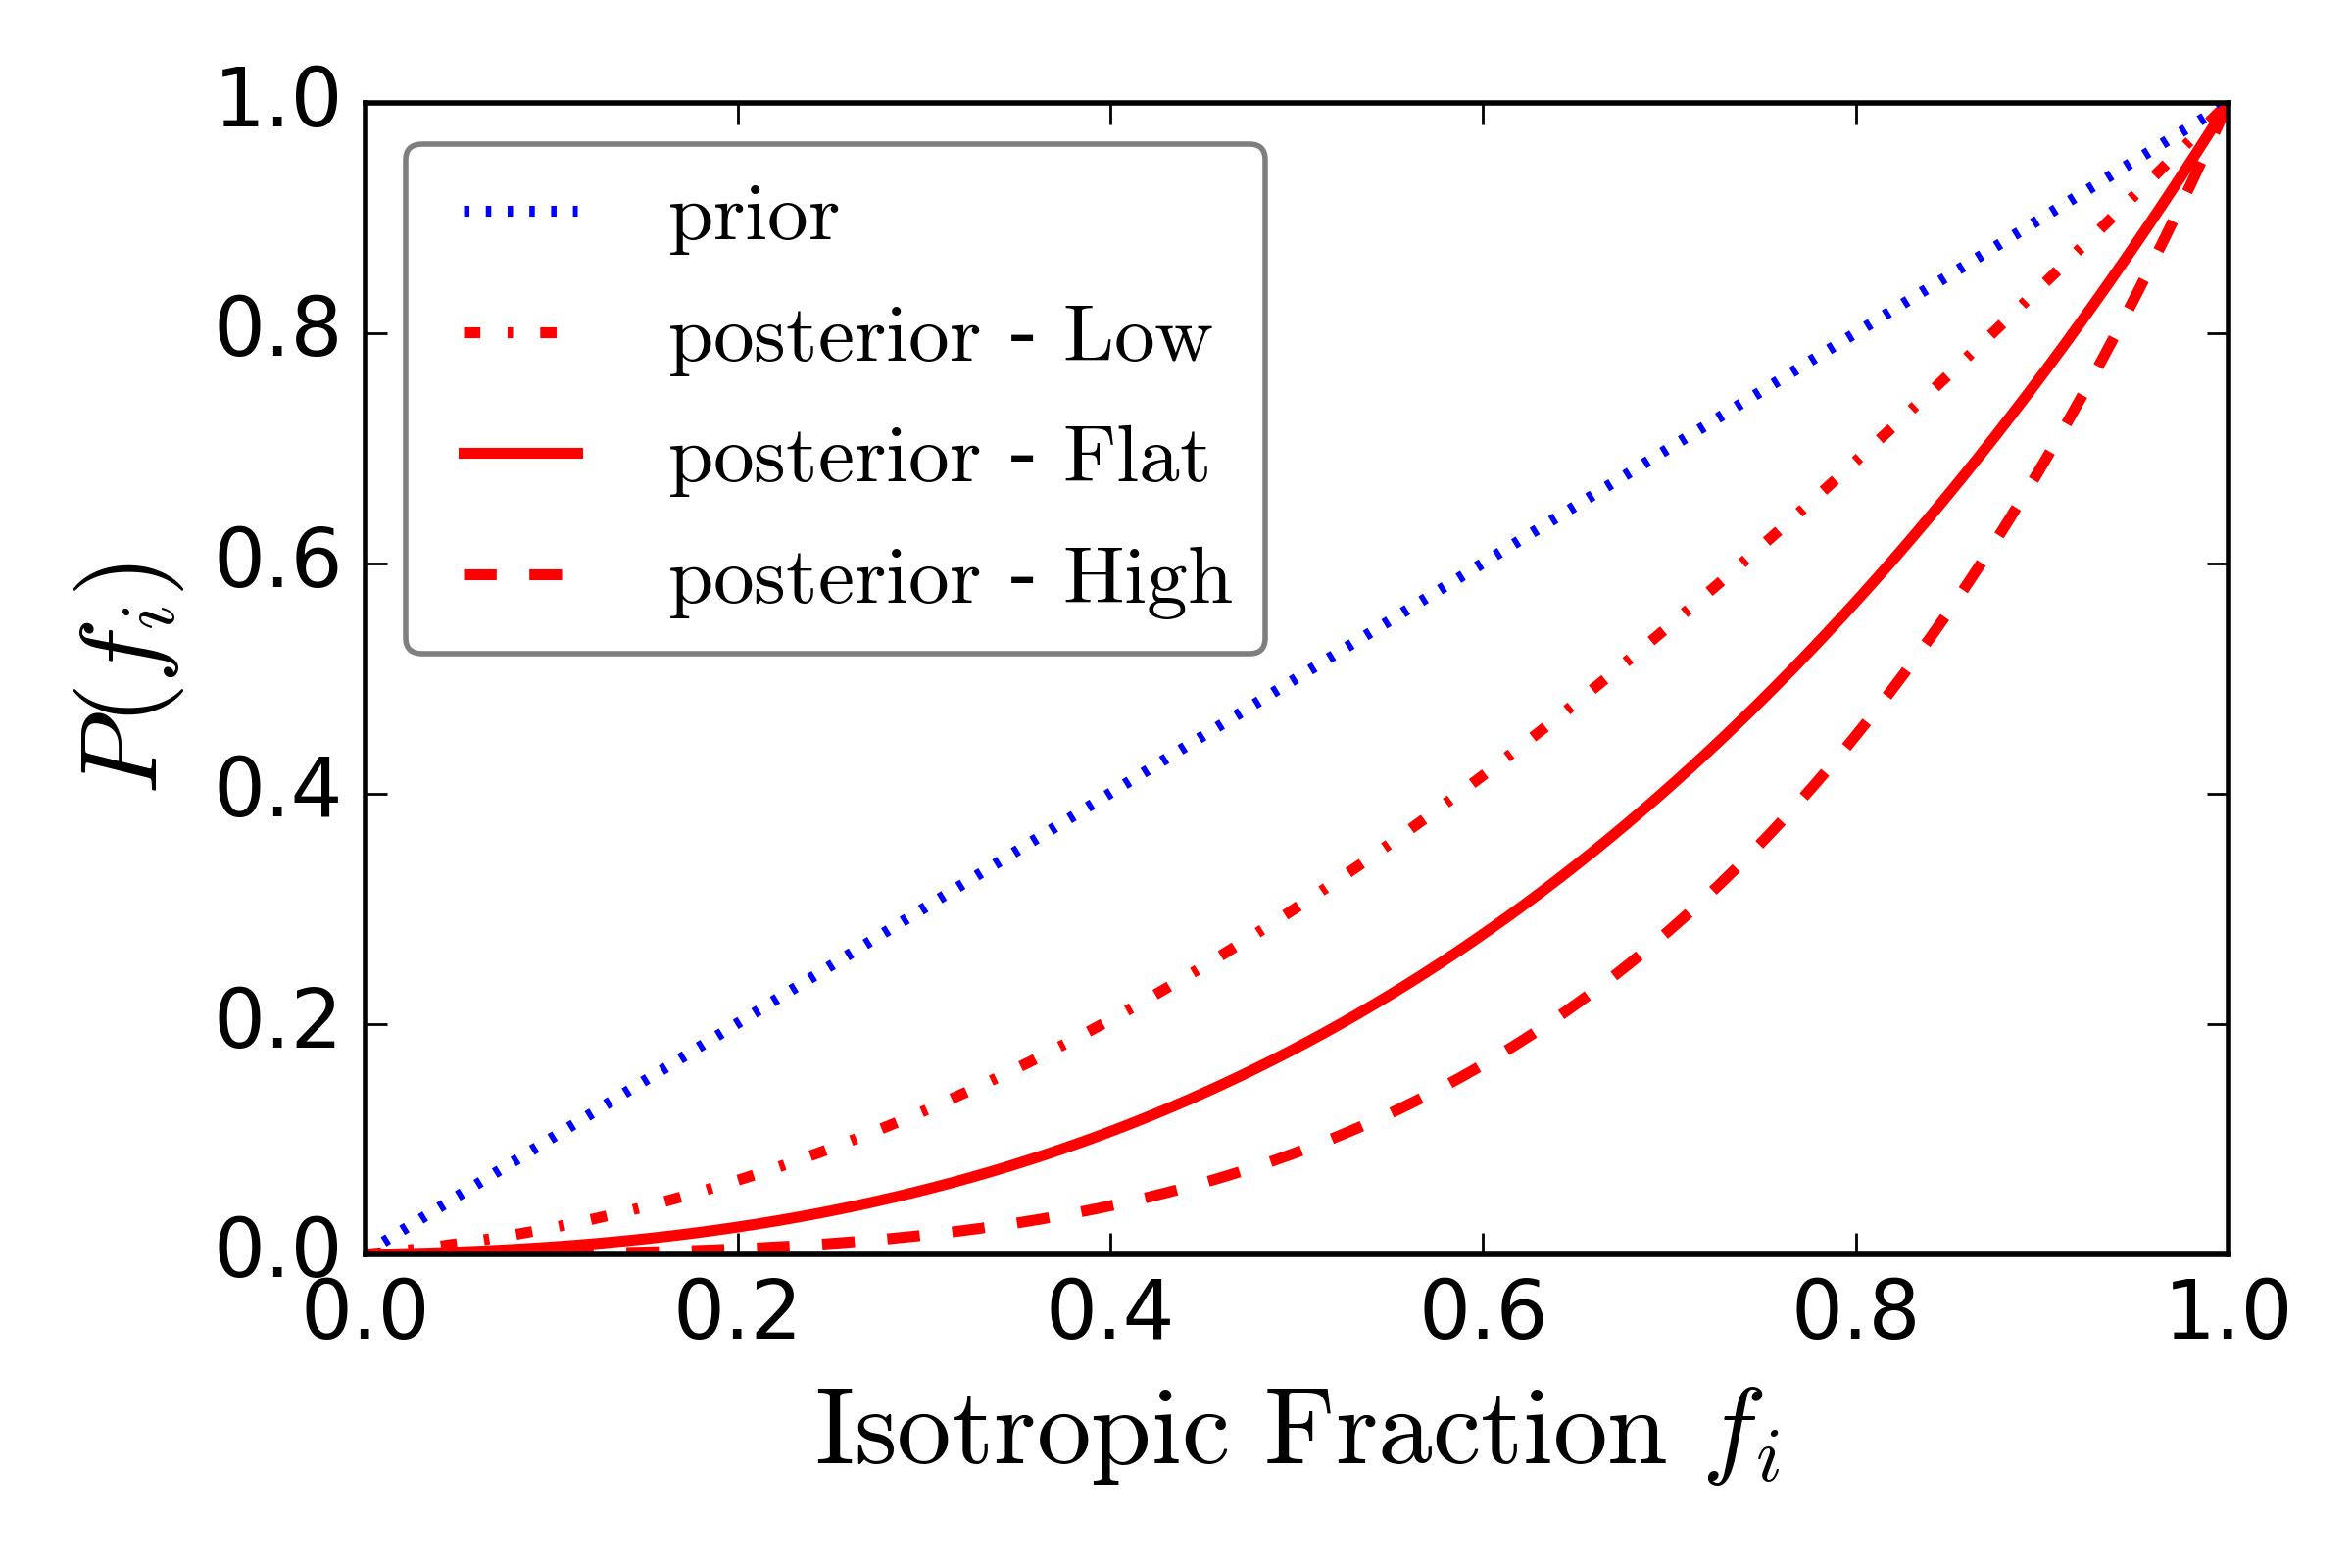
\includegraphics[width=0.45\textwidth]{../plots/isotropic_fraction_cumulative_posterior.png}
%\caption{\textbf{Fraction of the BBH population coming from an isotropic distribution} The dotted (blue) line shows the cumulative distribution for the flat prior on the fraction of BBHs coming from an isotropic distribution $f_i$. The solid (red) line shows the cumulative distribution for the posterior after O1, assuming that all BHs have their spin magnitude drawn from a uniform distribution. The dashed line assumes a `increasing' distribution $p(a) = 2a$ for BH spin magnitudes, whilst the dot-dash line assumes a `decreasing' distribution $p(a) = 2(1-a)$. We see that regardless of our assumption regarding BH spin magnitudes, there is a preference for a large fraction coming from an isotropic distribution.}
%\label{fig:mixture_fraction_posterior}
%\end{figure}
%

We fit a mixture model (labelled model 'M') where a fraction $f_i$ ($f_i=\lambda$ in the derivations above) of BBHs have spins drawn from an isotropic distribution, whilst a fraction $1 - f_i$ have their spins aligned with the orbital angular momentum. We assume a flat prior on the fraction $f_i$. To test the robustness of our result, we vary the distribution we assume for BH spin magnitude distributions as with the aligned and isotropic models. We use the `uniform', `increasing' and `decreasing' distributions introduced in Section X, assuming all BHs have their spin magnitude drawn from the same distribution. We calculate the posterior given by EquationX plot the posterior distribution/cumulative posterior in Figure~\ref{fig:mixture_fraction_posterior}. We find the mean fraction of BBHs coming from an isotropic distribution is 0.63, 0.71 and 0.78 assuming the `decreasing', `uniform' and `increasing' distributions for spin magnitudes respectively, compared to the prior mean of 0.5. The lower 90\% limits are 0.26, 0.39 and 0.52 respectively, compared to the prior of 0.1. Thus, irrespective of our ignorance of the BH spin magnitude distribution, we find that the current O1 LIGO observations constrain the majority of BBHs to have their spins drawn from an isotropic distribution. 

If we assume that the subpopulation of BBHs with isotropically distributed spin orientations corresponds to a subpopulation of dynamically formed BBHs, our result suggests that the majority of merging BBHs observed by LIGO are formed dynamically, rather than through isolated binary evolution.

The evidence ratios of these models to the isotropic distribution with uniform spin magnitudes are 0.85, 0.39 and 0.19. Thus we cannot rule out a mixture with the current data. 


\section{Hierarchical Modelling} 
\label{sec:hierarchical}

LIGO measures $\chieff$ better than any other spin parameter, but
still with significant uncertainty, so we need to properly incorporate
measurement uncertainty in our analysis; thus our analysis must be
\emph{hierarchical} \citep{2010ApJ...725.2166H,2010PhRvD..81h4029M}.
In a hierarchical analysis, we assume that each event has a true, but
unknown, value of the effective spin, drawn from the population
distribution, which may have some parameters $\lambda$; then the
system is observed, represented by the likelihood function, which
results in a distribution for the true effective spin (and all other
paremeters describing the system) consistent with the data.
Combining, the joint posterior on each system's $\chieff^i$ parameters
and the population parameters $\lambda$ implied by a set of
observations each with data $d^i$, is
\begin{equation}
  p\left( \left\{ \chieff^i \right\}, \lambda \mid \left\{ d^i \right\} \right) \propto \left[ \prod_{i=1}^{N_\mathrm{obs}} p\left(d^i \mid \chieff^i \right) p\left( \chieff^i \mid \lambda \right) \right] p\left(\lambda\right).
\end{equation}

The components of this formula are
\begin{itemize}
\item The GW (marginal) likelihood, $p\left(d \mid \chieff\right)$.
  ``Marginal'' because we are (implicitly) integrating over all
  parameters of the signal but $\chieff$.  Note that it is the
  likelihood, not the posterior that matters for the hierarchical
  analysis; if we are given posterior distributions or posterior
  samples, we need to re-weight to "remove" the prior and obtain the
  likelihood.
\item The population distribution for $\chieff$,
  $p\left( \chieff \mid \lambda \right)$.  This function can be
  parameterised by population-level parameters, $\lambda$.  (In the
  cases discussed above, there are no parameters for the population.)
\item The prior on the population-level parameters, $p(\lambda)$.
\end{itemize}
If we don't care about the individual event $\chieff$ paremetrs, we
can integrate them out, obtaining
\begin{equation}
  p\left( \lambda \mid \left\{ d^i \right\} \right) \propto \left[ \prod_{i=1}^{N_\mathrm{obs}} \int \dd \chieff^i \, p\left(d^i \mid \chieff^i \right) p\left( \chieff^i \mid \lambda \right) \right] p\left(\lambda\right).
\end{equation}
If we are given posterior samples of $\chieff^{ij}$ ($i$ labels the
event, $j$ labels the particular posterior sample) drawn from an
analysis using a prior $p\left( \chieff \right)$, then we can
approximate the integral by an re-weighted average of the population
distribution over the samples (here $p\left( \chieff^{ij} \right)$ is
the prior used to produce the posterior samples):
\begin{equation}
  p\left( \lambda \mid \left\{ d^i \right\} \right) \propto \left[ \prod_{i=1}^{N_\mathrm{obs}} \frac{1}{N_i} \sum_{j=1}^{N_i} \frac{p\left( \chieff^{ij} \mid \lambda \right)}{p\left( \chieff^{ij} \right)} \right] p\left(\lambda\right).
\end{equation}

\section{Mass Ratio}
\label{sec:mass-ratio}

\will{Some plots go here showing how the distribution changes as a
  function of mass ratio.}

\bibliography{AlignedIsotropicGW}

\end{document}

